\section{ダイレクトティーチング}
\label{sec:direct_teaching}

\subsection{手順}
ダイレクトティーチングとは,手動で手先を動かし,2 軸ロボットにその動きを再現させることである.ダイレクトティーチングを行うためには,以下のステップを実行すればよい.

\underline{\textbf{ステップ 1}}\quad 
手先位置 $P_3$ が所望の軌道に沿うように手先を手で動かし,関節角 $\theta_x(t)$,$\theta_y(t)$(あるいは手先位置 $x(t)$,$y(t)$)をデータとして取得する.

\underline{\textbf{ステップ 2}}\quad 
ステップ 1 で取得した教師データを目標値 $\theta_x^{\mathrm{ref}}(t)$,$\theta_y^{\mathrm{ref}}(t)$(あるいは $x^{\mathrm{ref}}(t)$,$y^{\mathrm{ref}}(t)$)として手先位置($x(t)$,$y(t)$)の動きを再現する.

\subsection{実験}
\label{sec:teach}

\subsubsection{教師データの取得}

教師データを取得するため,図\ref{fig:ex_robot_teach} に示す実機実験モデル ``ex\_robot\_teach.slx'' を作成し,\verb|¥teach| に保存する.また,\ref{sec:armpara} 節で示した M ファイル ``armpara.m'',\ref{sec:sim_pd_exp} 節で示した M ファイル ``armIPD.m'',\ref{sec:xy_control_const} 節で作成した M ファイル ``sim\_anime.m'' および \ref{sec:sim_data_input} 節で作成した ``sim\_robot\_xy2.slx'',``ex\_robot\_xy2.slx'' を \verb|¥teach| に保存する.

\begin{figure}[H]
    \centering
    \begin{subfigure}[b]{0.48\linewidth}
        \centering
        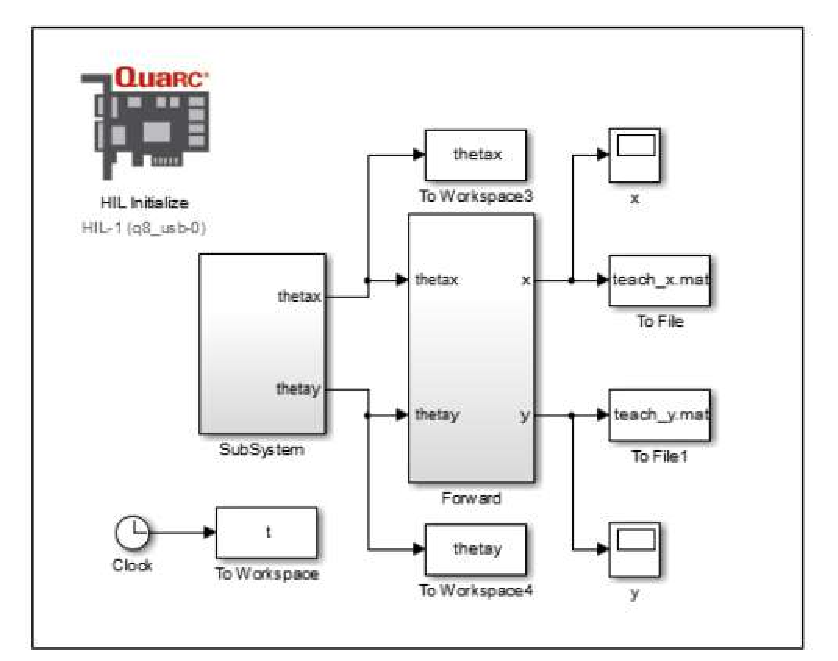
\includegraphics[width=\linewidth]{figure/ex_robot_teach.pdf}
        \caption{実機実験モデル ``ex\_robot\_teach.slx''}
    \end{subfigure}
    \begin{subfigure}[b]{0.48\linewidth}
        \centering
        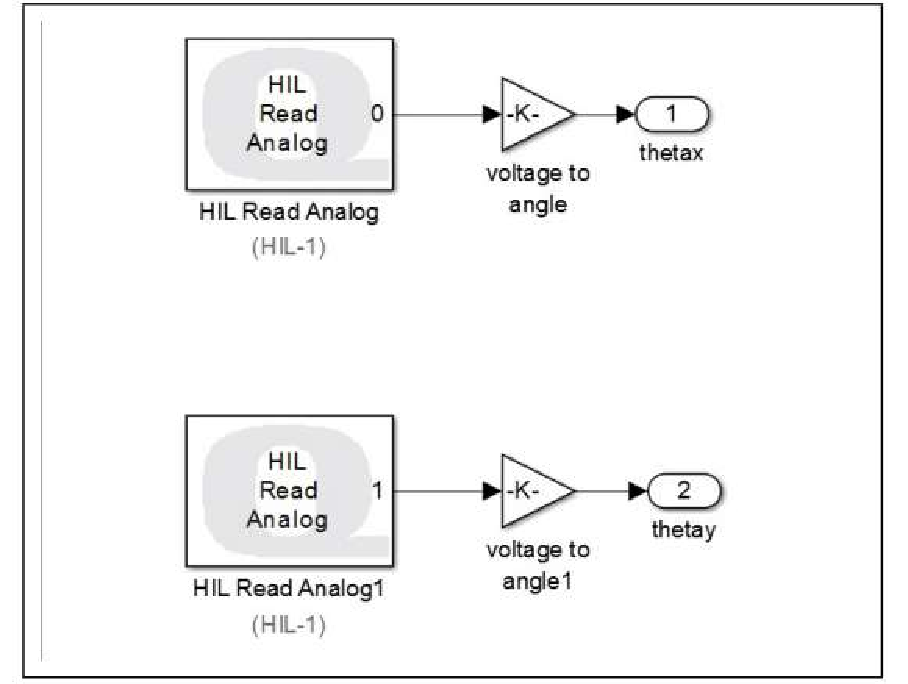
\includegraphics[width=\linewidth]{figure/ex_robot_teach_subsystem.pdf}
        \caption{Subsystem ``2D Robot'' の内容}
    \end{subfigure}
    \caption{教師データ取得のための実機実験モデル ``ex\_robot\_teach.slx''}
    \label{fig:ex_robot_teach}
\end{figure}

つぎに,``ex\_robot\_teach.slx'' はデータ取得は30秒間であることに注意し,``Start''アイコンをクリックした後,所望の軌道に沿うように手先を動かす.実験終了後,プロットされたデータが ``teach\_x.mat'',``teach\_y.mat'' という名前で \verb|¥teach| に保存されていることを確認する.

つぎに,“\texttt{ex\_robot\_teach.slx}” はデータ取得は30秒間であることに注意し,“Start” アイコンをクリックした後,所望の軌道に沿うように手先を動かす.実験終了後,プロットされたデータが “\texttt{teach\_x.mat}”, “\texttt{teach\_y.mat}” という名前で \texttt{\textbackslash teach} に保存されていることを確認する.

以上の作業が終了した後,\textbf{MATLAB Command Window} で

\begin{lstlisting}[language=Matlab]
load teach_x;
load teach_y;
x_ref_data = teach_x(2,:);    % x_ref の取得
y_ref_data = teach_y(2,:);    % y_ref の取得
t_data     = teach_x(1,:);    

figure(1); plot(t_data,x_ref_data,t_data,y_ref_data);
xlabel('time [s]'); ylabel('{¥it y}^{ref} [m] and {¥it x}^{ref} [m]');

figure(2); plot(x_ref_data,y_ref_data);
xlabel('{¥it x}^{ref} [m]'); ylabel('{¥it y}^{ref} [m]');
\end{lstlisting}

のように入力すると,取得された教師データが図\ref{fig:teaching_data}のように表示される.

\begin{figure}[H]
    \centering
    \begin{subfigure}[b]{0.45\linewidth}
        \centering
        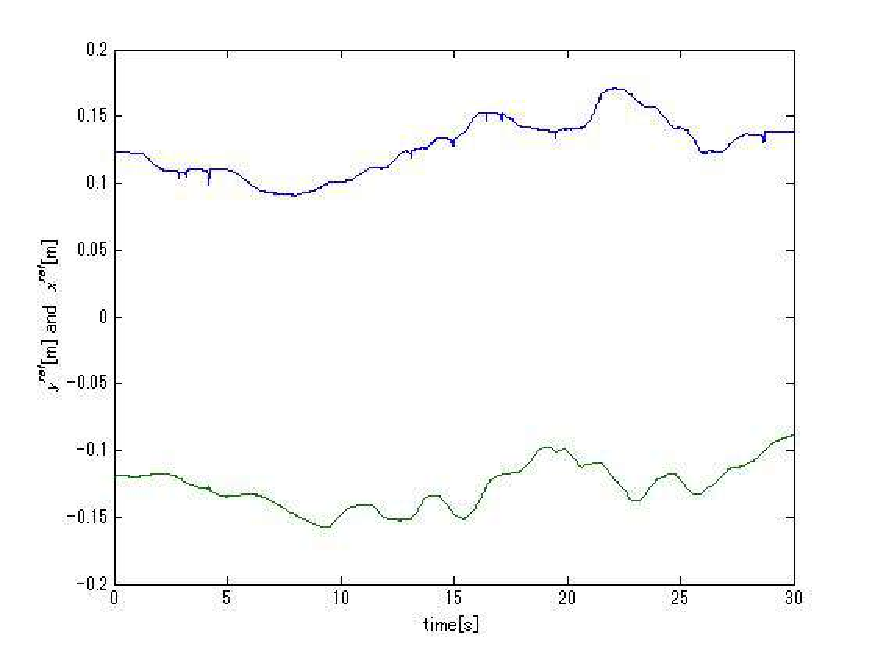
\includegraphics[width=\linewidth]{figure/fig1_xref_yref.pdf}
        \caption{$x^{\mathrm{ref}}(t),\ y^{\mathrm{ref}}(t)$}
    \end{subfigure}
    \begin{subfigure}[b]{0.45\linewidth}
        \centering
        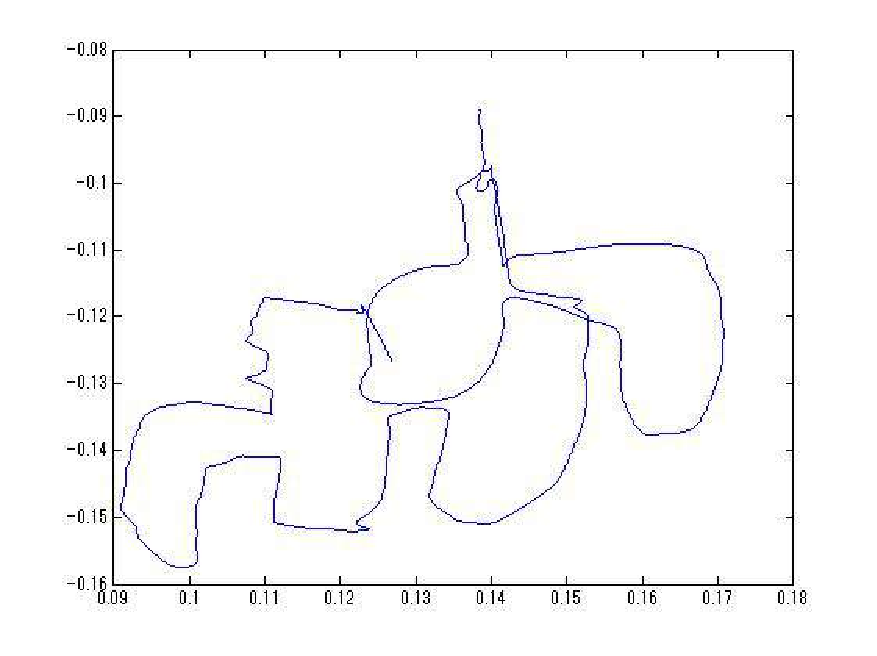
\includegraphics[width=\linewidth]{figure/dairekuto1.pdf}
        \caption{$x$--$y$ 平面での表示}
    \end{subfigure}
    \caption{取得された教師データ}
    \label{fig:teaching_data}
\end{figure}


\noindent
\textbf{ステップ2}: \quad
まず,MATLAB Command Window で以下のように入力し,パラメータおよび目標値を設定する.

\begin{lstlisting}[language=Matlab]
armIPD
各パラメータを設定して下さい
omegaMx = 20
omegaMy = 20
........................................................... 《略》 ...........................................................
alphaM1x = 2
alphaM2x = 2
alphaM1y = 2
alphaM2y = 2
........................................................... 《略》 ...........................................................
load teach_x; x_ref_data = x; 
load teach_y; y_ref_data = y; 
load teach_t; t_data = t;
\end{lstlisting}

つぎに,ステップ1で取得した教師データを目標値($x^{\mathrm{ref}}, y^{\mathrm{ref}}$)として “\texttt{sim\_robot\_xy2.slx}” によりシミュレーションを行い,以下のように入力してシミュレーション結果をアニメーション表示する(図\ref{fig:direct_teaching_anim}).

\noindent
MATLAB Command Window で

\begin{lstlisting}[language=Matlab]
sim_anime;
\end{lstlisting}

と入力してアニメーションにより各リンクに無理な動きがないことを確認した後,“\texttt{ex\_robot\_xy2.slx}” をコンパイルして実機実験を行う.その結果,図\ref{fig:direct_teaching_result} の実験結果が得られる.

\begin{figure}[H]
    \centering
    \begin{subfigure}[b]{0.45\linewidth}
        \centering
        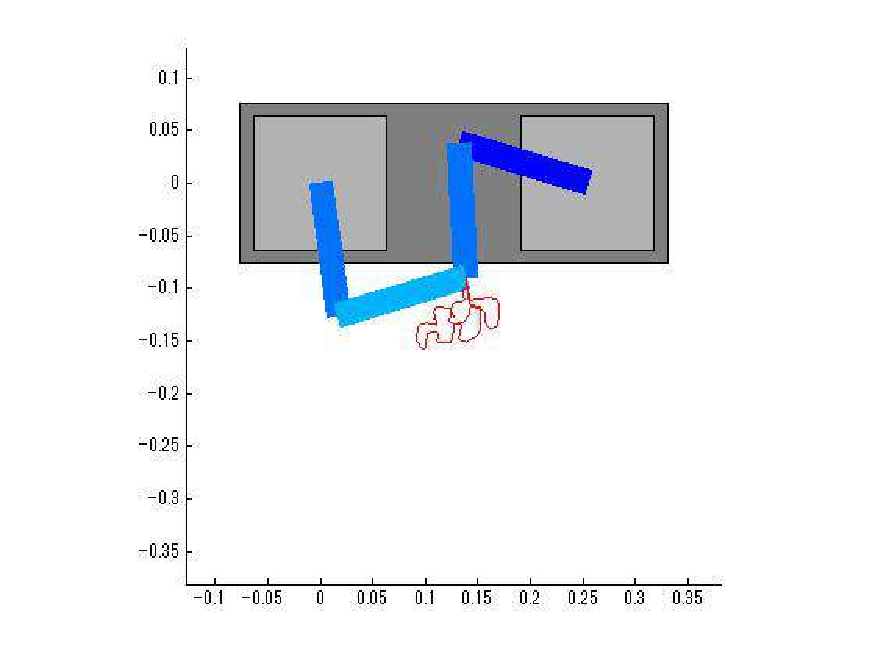
\includegraphics[width=\linewidth]{figure/dairekuto_anime.pdf}
        \caption{シミュレーション結果のアニメーション表示}
        \label{fig:direct_teaching_anim}
    \end{subfigure}
    \begin{subfigure}[b]{0.45\linewidth}
        \centering
        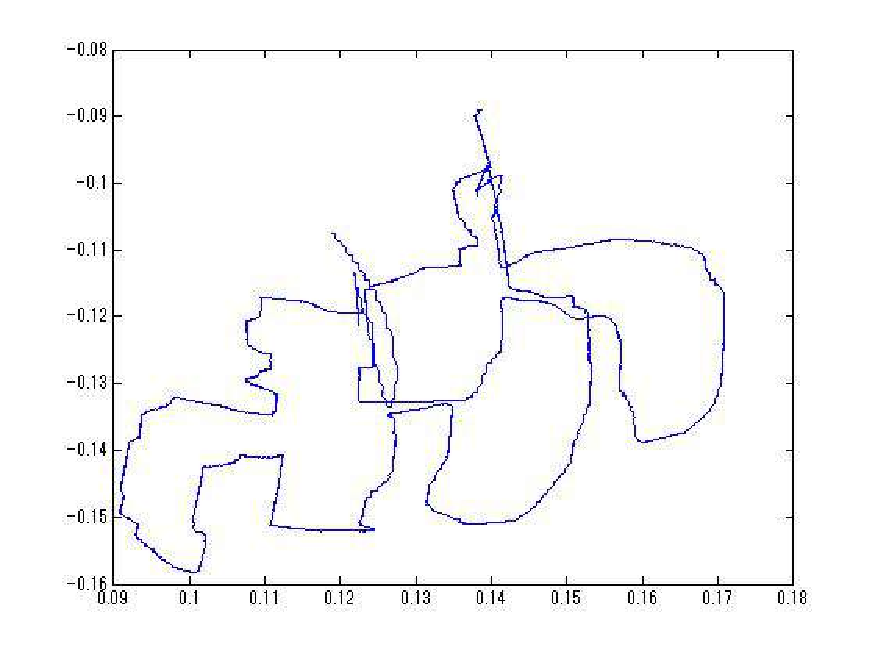
\includegraphics[width=\linewidth]{figure/ex_kekka.pdf}
        \caption{ダイレクトティーチングの実験結果}
        \label{fig:direct_teaching_result}
    \end{subfigure}
    \caption{ダイレクトティーチングにおけるアニメーションと実験結果}
\end{figure}
